\chapter{Supplementary Material}

\section{Material from original PGExplainer}
\label{sec:PGE_material}

\begin{algorithm}
    \caption{Training Algorithm for Explaining Node Classification from \cite{luo2020parameterized}.}
    \label{alg:node-alg}
    \begin{algorithmic}[1]
    \REQUIRE Input graph $G_o = (\mathcal{V}, \mathcal{E})$, node features $X$, node labels $Y$, set of instances to be explained $\mathcal{I}$, trained GNN model: $\text{GNNE}_{\Phi_0}(\cdot)$ and $\text{GNNC}_{\Phi_1}(\cdot)$, parameterized explainer MLP $\Psi$.
    \FOR{each node $i \in \mathcal{I}$}
        \STATE $G^{(i)}_o \leftarrow$ extract the computation graph for node $i$.
        \STATE $Z^{(i)} \leftarrow \text{GNNE}_{\Phi_0}(G^{(i)}_o, X)$.
        \STATE $Y^{(i)} \leftarrow \text{GNNC}_{\Phi_1}(Z^{(i)})$.
    \ENDFOR
    \FOR{each epoch}
        \FOR{each node $i \in \mathcal{I}$}
            \STATE $\Omega \leftarrow$ latent variables calculated with (10).
            \FOR{$k \leftarrow 1$ to $K$}
                \STATE $G^{(i,k)}_s \leftarrow$ sampled from (4).
                \STATE $\hat{Y}^{(i,k)}_s \leftarrow \text{GNNC}_{\Phi_1}(\text{GNNE}_{\Phi_0}(G^{(i,k)}_s, X))$.
            \ENDFOR
        \ENDFOR
        \STATE Compute loss with (9).
        \STATE Update parameters $\Psi$ with backpropagation.
    \ENDFOR
    \end{algorithmic}
    \end{algorithm}
    
    \vspace{0.5cm}
    
    \begin{algorithm}
    \caption{Training Algorithm for Explaining Graph Classification from \cite{luo2020parameterized}.}
    \label{alg:graph-alg}
    \begin{algorithmic}[1]
    \REQUIRE A set of input graphs with $i$-th graph represented by $G^{(i)}_o$, node features $X^{(i)}$, label $Y^{(i)}$, trained GNN model: $\text{GNNE}_{\Phi_0}(\cdot)$ and $\text{GNNC}_{\Phi_1}(\cdot)$, parameterized explainer MLP $\Psi$.
    \FOR{each graph $G^{(i)}_o$}
        \STATE $Z^{(i)} \leftarrow \text{GNNE}_{\Phi_0}(G^{(i)}_o, X^{(i)})$.
        \STATE $Y^{(i)} \leftarrow \text{GNNC}_{\Phi_1}(Z^{(i)})$.
    \ENDFOR
    \FOR{each epoch}
        \FOR{each graph $G^{(i)}_o$}
            \STATE $\Omega \leftarrow$ latent variables calculated with (11).
            \FOR{$k \leftarrow 1$ to $K$}
                \STATE $G^{(i,k)}_s \leftarrow$ sampled from (4).
                \STATE $\hat{Y}^{(i,k)}_s \leftarrow \text{GNNC}_{\Phi_1}(\text{GNNE}_{\Phi_0}(G^{(i,k)}_s, X^{(i)}))$.
            \ENDFOR
        \ENDFOR
        \STATE Compute loss with (9).
        \STATE Update parameters $\Psi$ with backpropagation.
    \ENDFOR
    \end{algorithmic}
\end{algorithm}

\begin{table}[h]
    \centering
    \scriptsize
    \begin{tabularx}{\linewidth}{l|X X X X|X X}
    \hline
    \textbf{Accuracy} & \textbf{BA-Shapes} & \textbf{BA-Community} & \textbf{Tree-Cycles} & \textbf{Tree-Grid} & \textbf{BA-2Motif} & \textbf{MUTAG} \\
    \hline
    \textbf{Training}   & 0.98 & 0.99 & 0.99 & 0.92 & 1.00 & 0.87 \\
    \textbf{Validation} & 1.00 & 0.88 & 1.00 & 0.94 & 1.00 & 0.89 \\
    \textbf{Testing}    & 0.97 & 0.93 & 0.99 & 0.94 & 1.00 & 0.87 \\
    \hline
    \end{tabularx}
    \caption[Accuracies of original GNN downstream task]{Compact accuracy table for Node and Graph Classification. Reprinted from \cite{luo2020parameterized}.}
    \label{tab:compact-accuracy}
\end{table}


\section{Data visualization}
\label{sec:data_vis}

\begin{figure}[H]
    \centering
    \begin{subfigure}[b]{0.4\textwidth}
        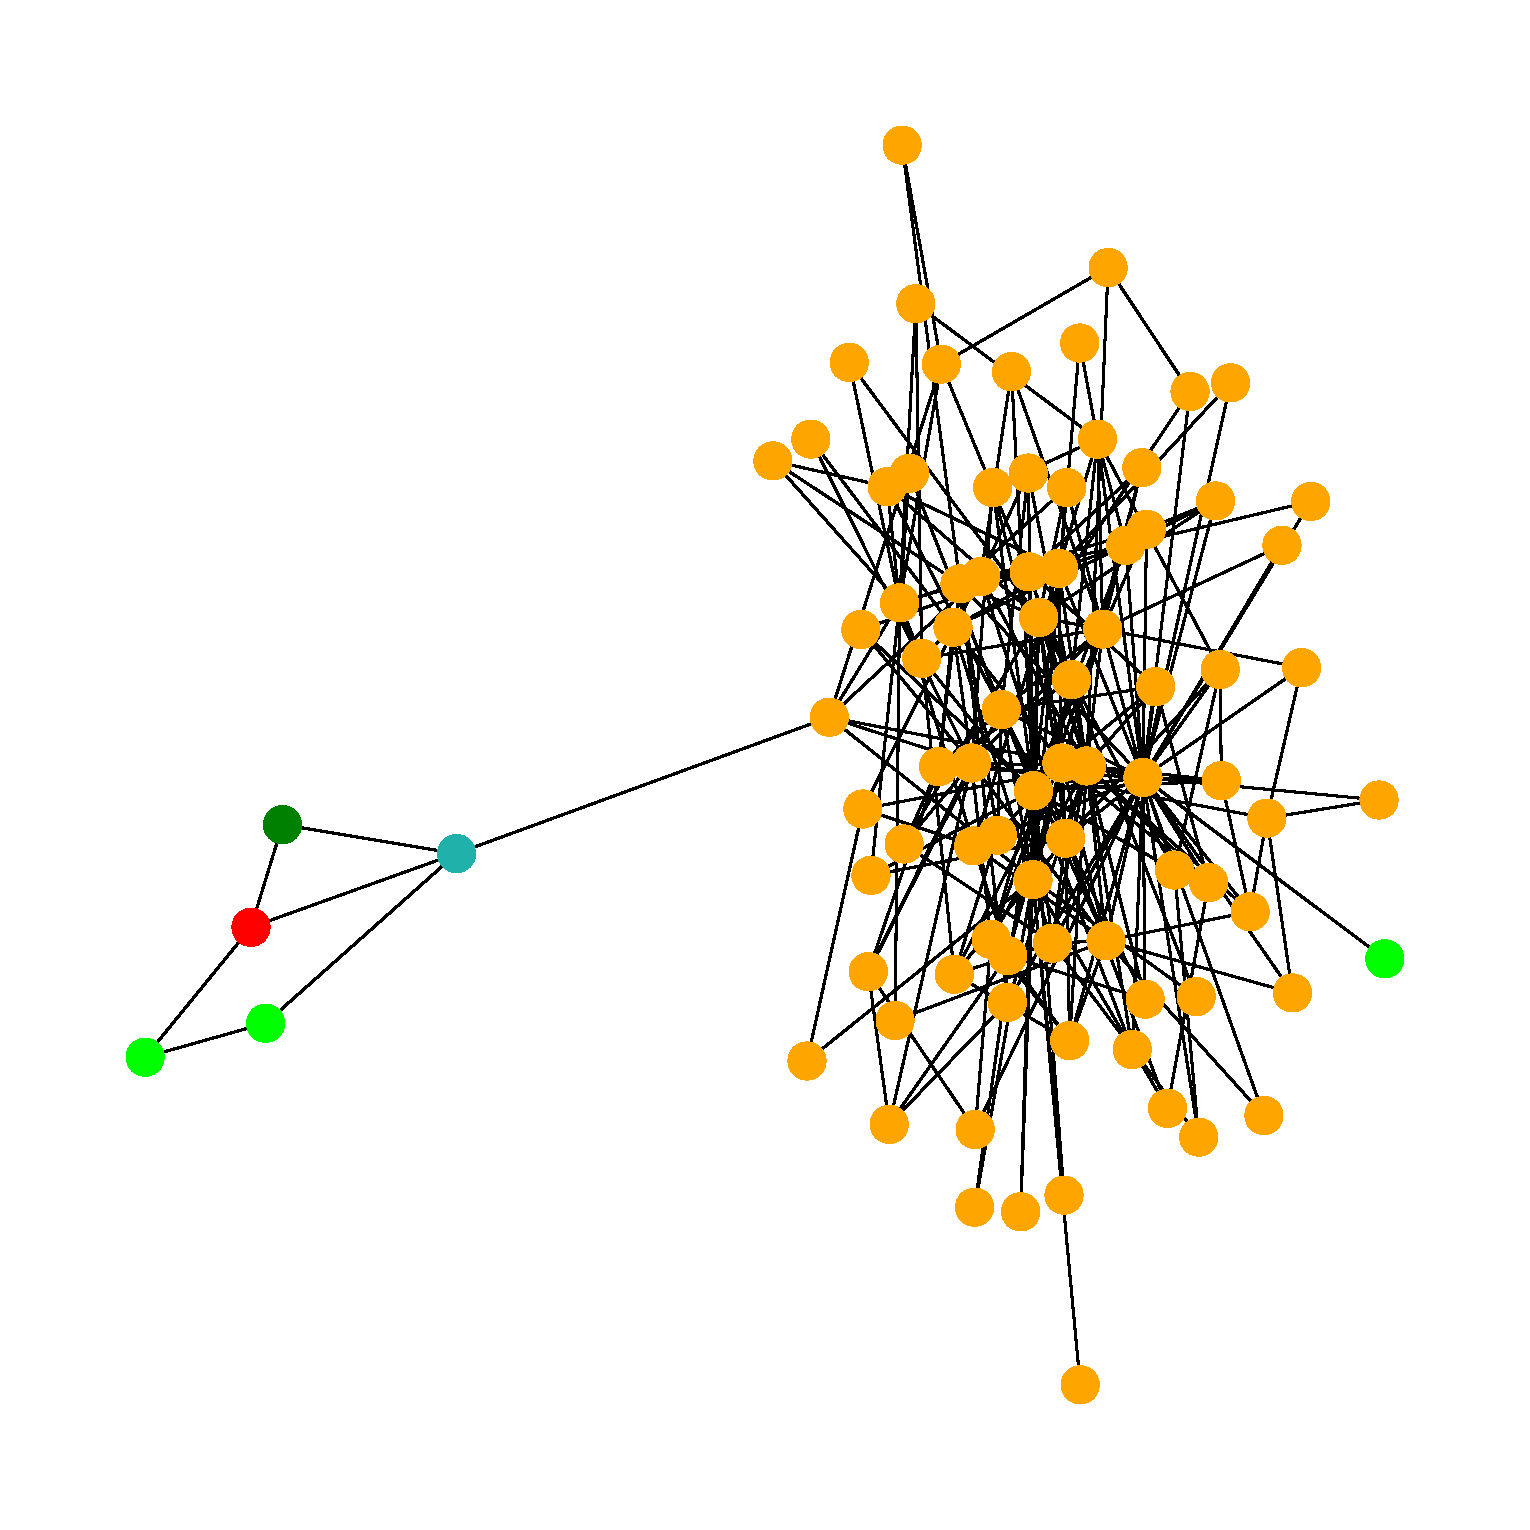
\includegraphics[width=\textwidth]{img/BA-Shapes-VIS-COMP-GRAPH.pdf}
        \caption{BA-Shapes}
    \end{subfigure}
    \hfill
    \begin{subfigure}[b]{0.4\textwidth}
        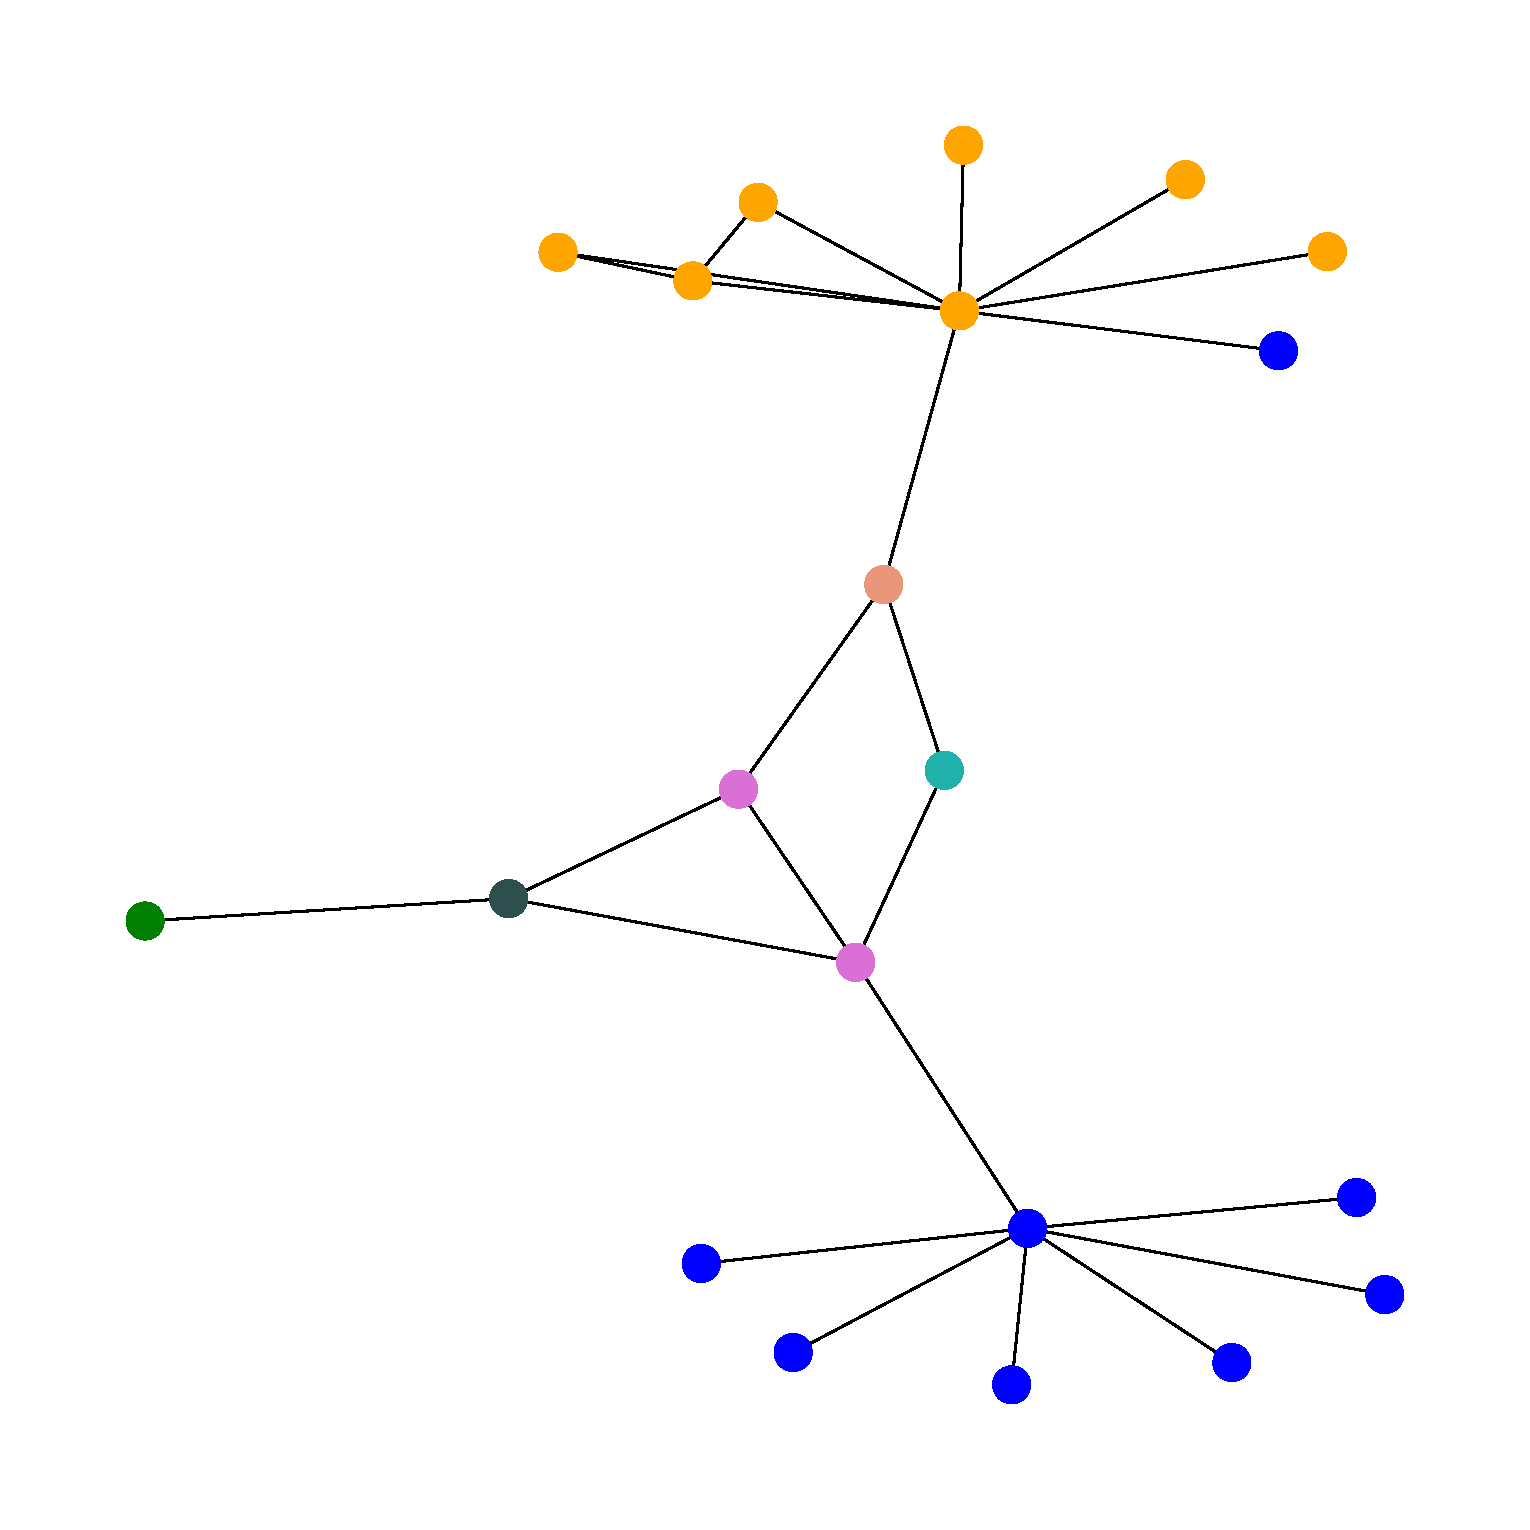
\includegraphics[width=\textwidth]{img/BA-Community-VIS-COMP-GRAPH.pdf}
        \caption{BA-Community}
    \end{subfigure}
    
    \vspace{0.5cm}
    
    \begin{subfigure}[b]{0.4\textwidth}
        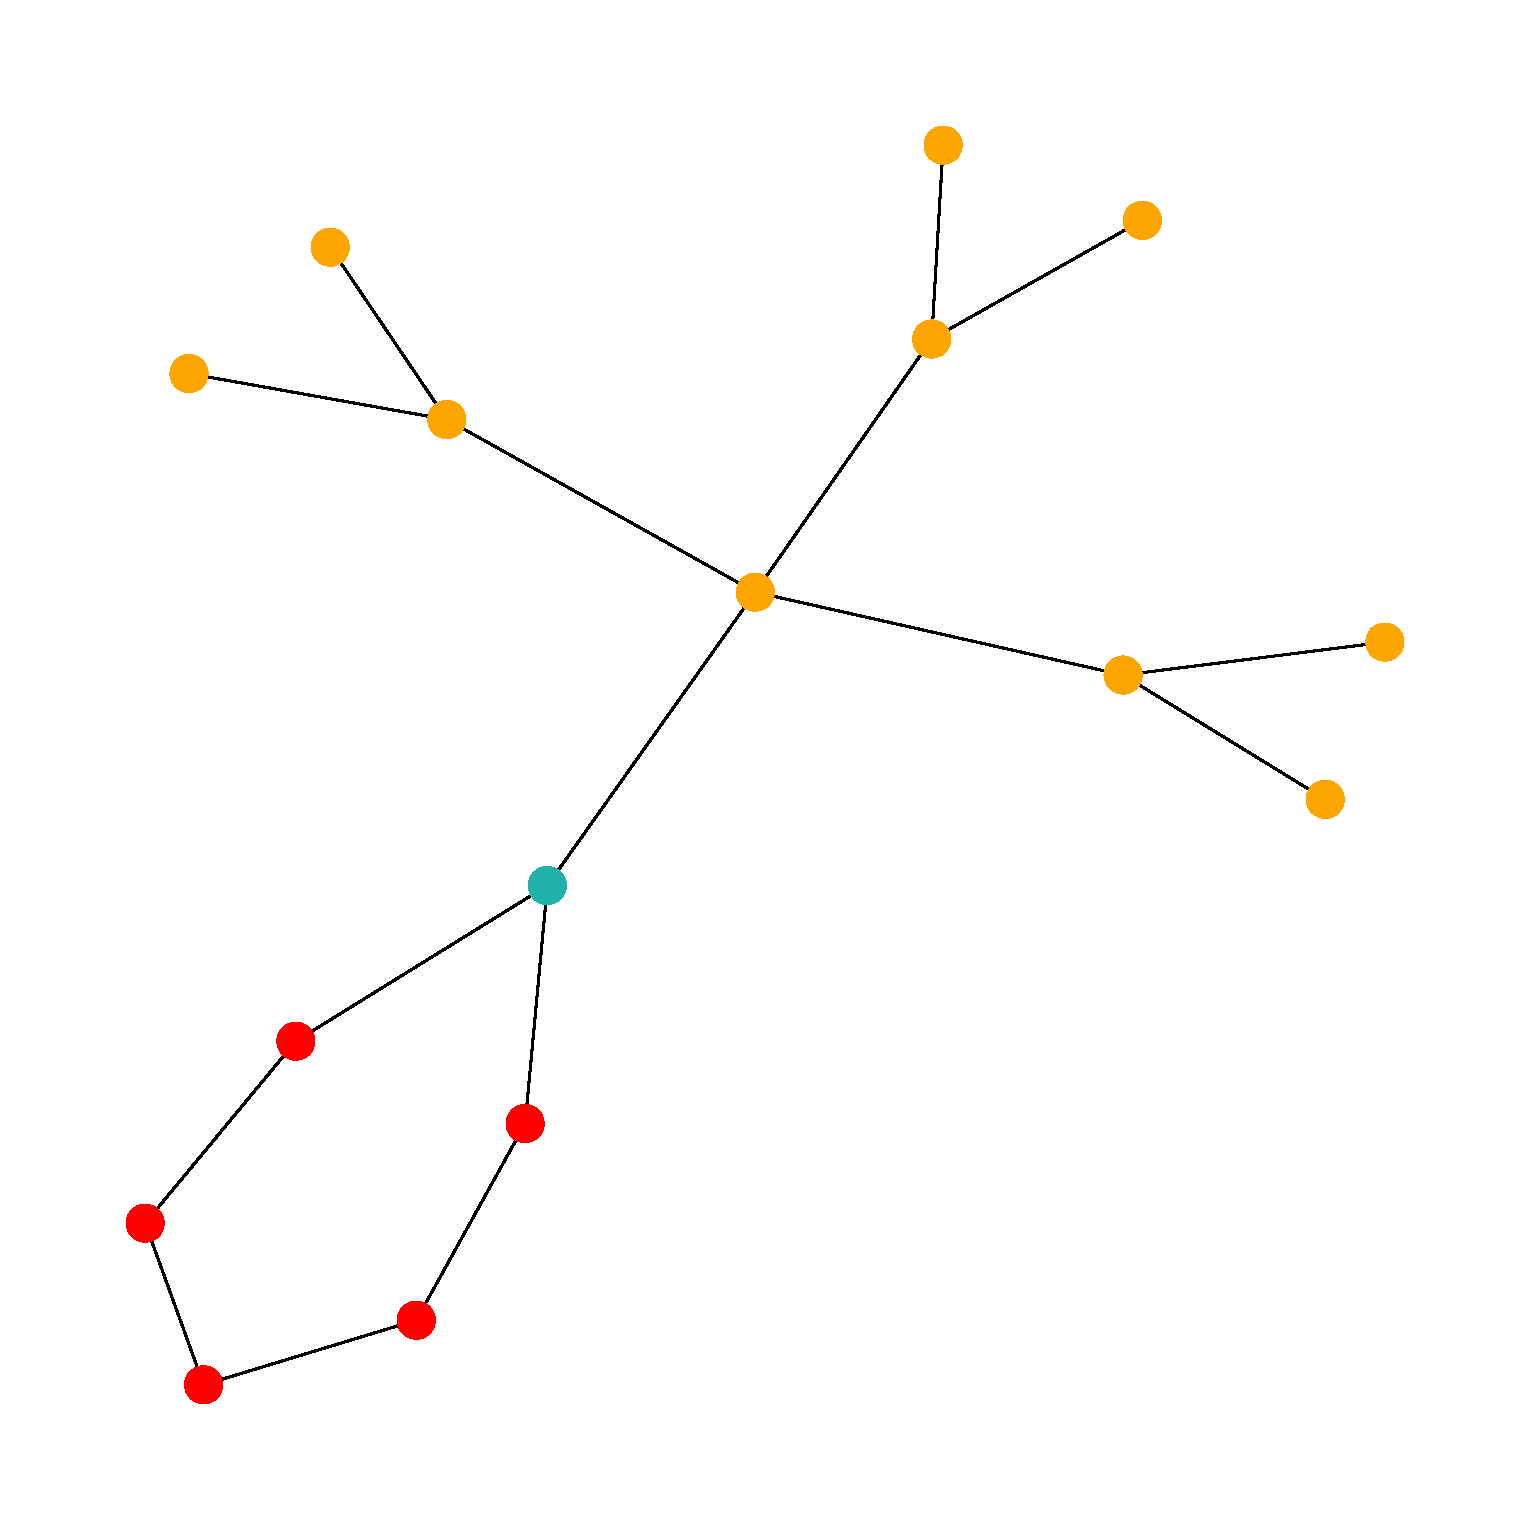
\includegraphics[width=\textwidth]{img/Tree-Cycles-VIS-COMP-GRAPH.pdf}
        \caption{Tree-Cycles}
    \end{subfigure}
    \hfill
    \begin{subfigure}[b]{0.4\textwidth}
        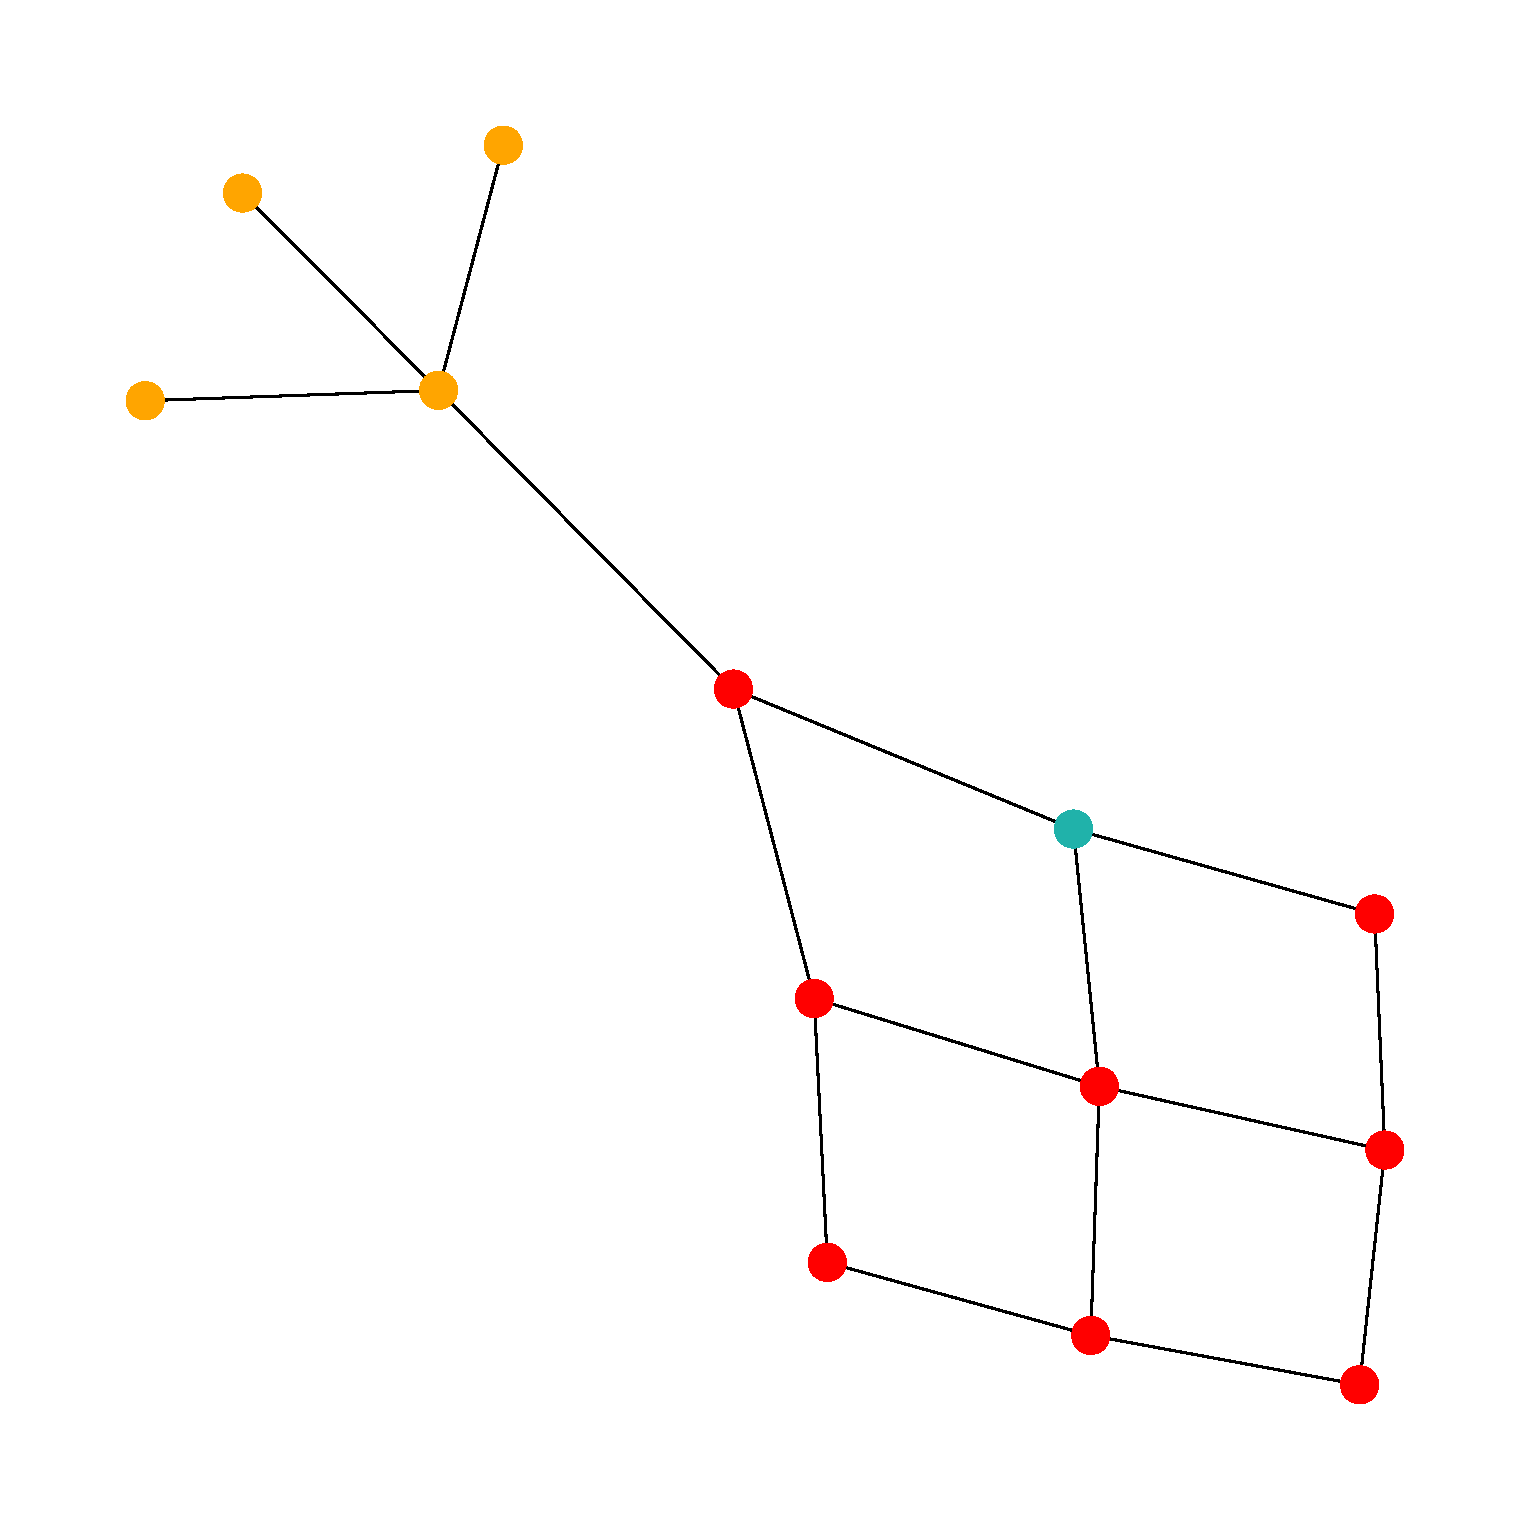
\includegraphics[width=\textwidth]{img/Tree-Grid-VIS-COMP-GRAPH.pdf}
        \caption{Tree-Grid}
    \end{subfigure}
    
    \vspace{0.5cm}
    
    \begin{subfigure}[b]{0.4\textwidth}
        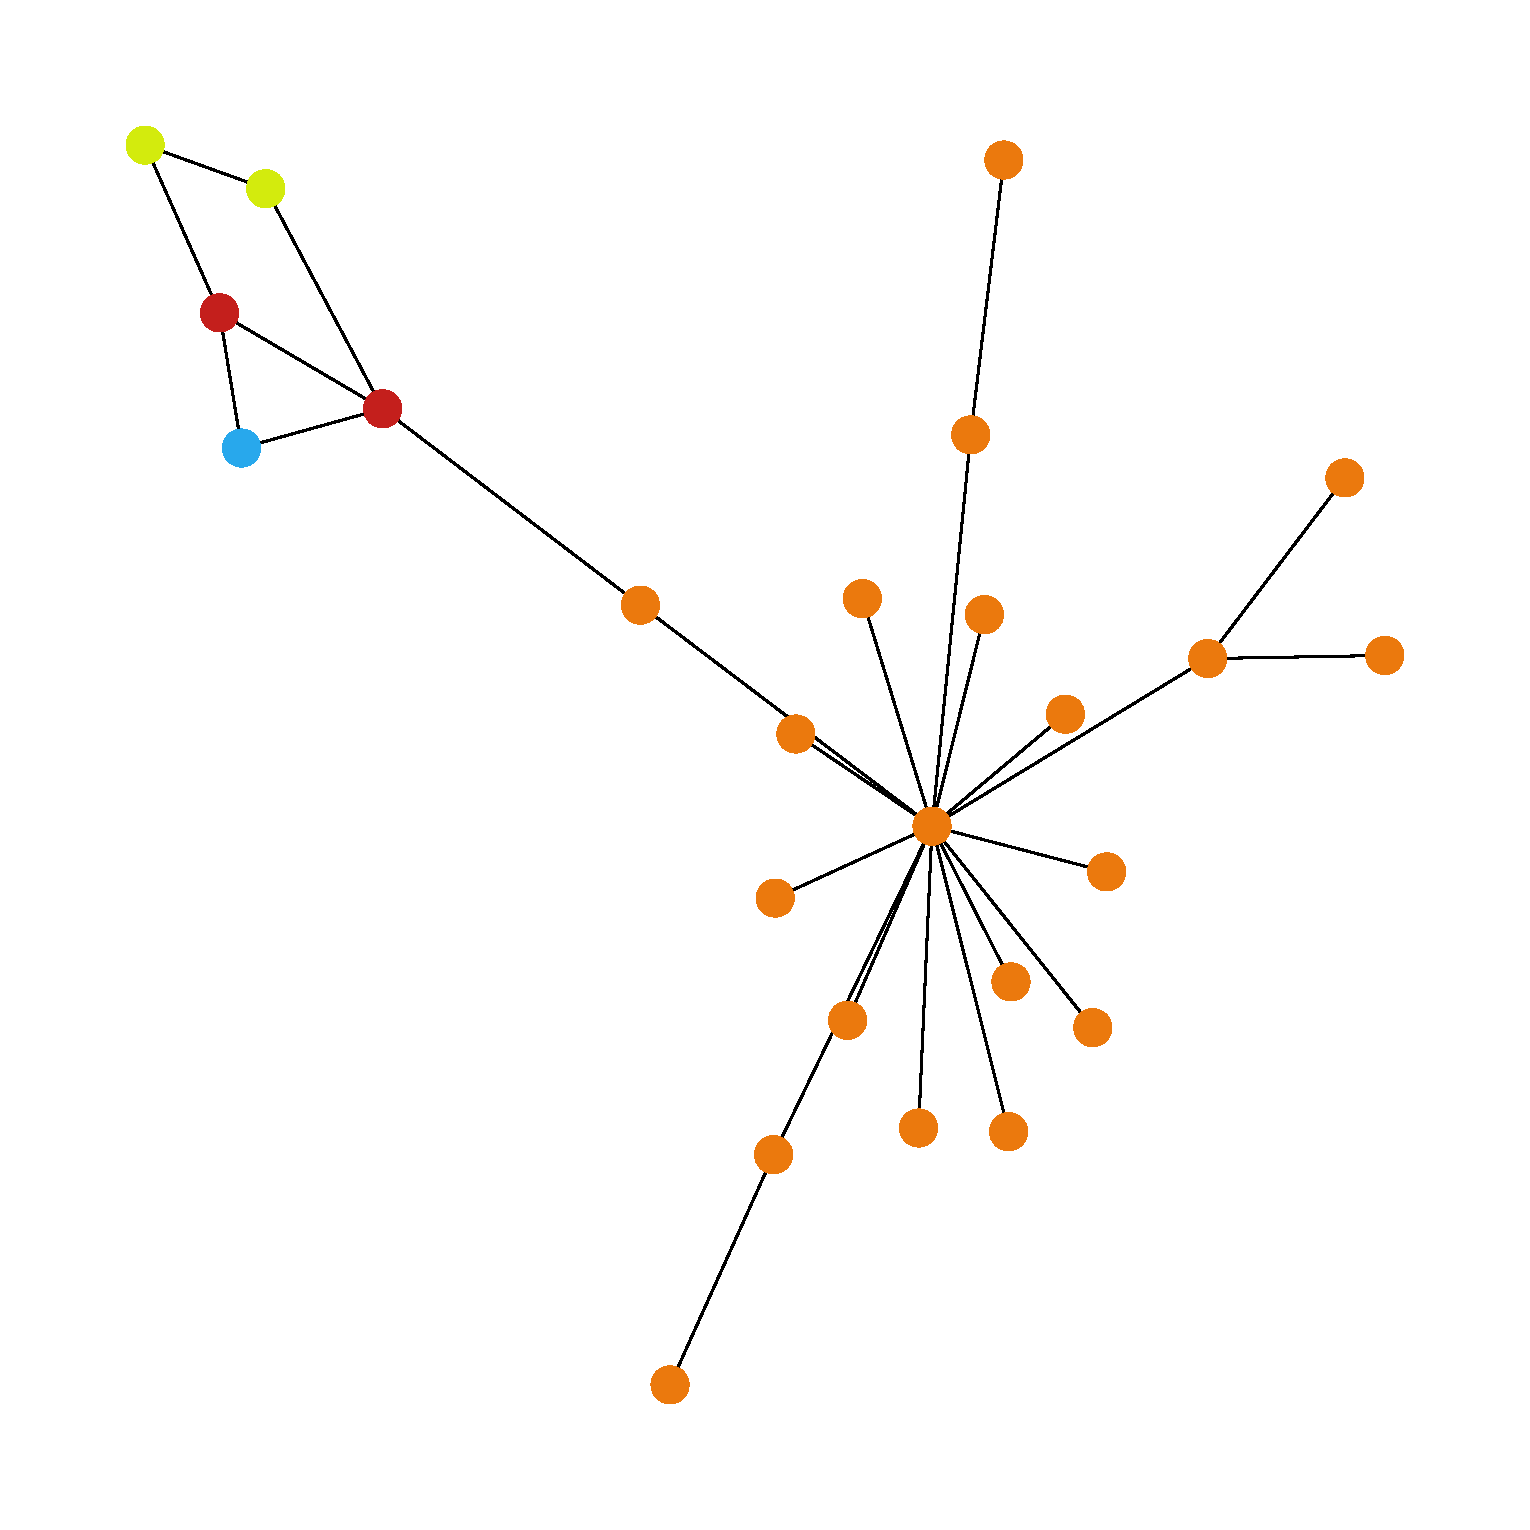
\includegraphics[width=\textwidth]{img/BA-2Motif-VIS-UNLABELED.pdf}
        \caption{BA-2Motif}
    \end{subfigure}
    \hfill
    \begin{subfigure}[b]{0.4\textwidth}
        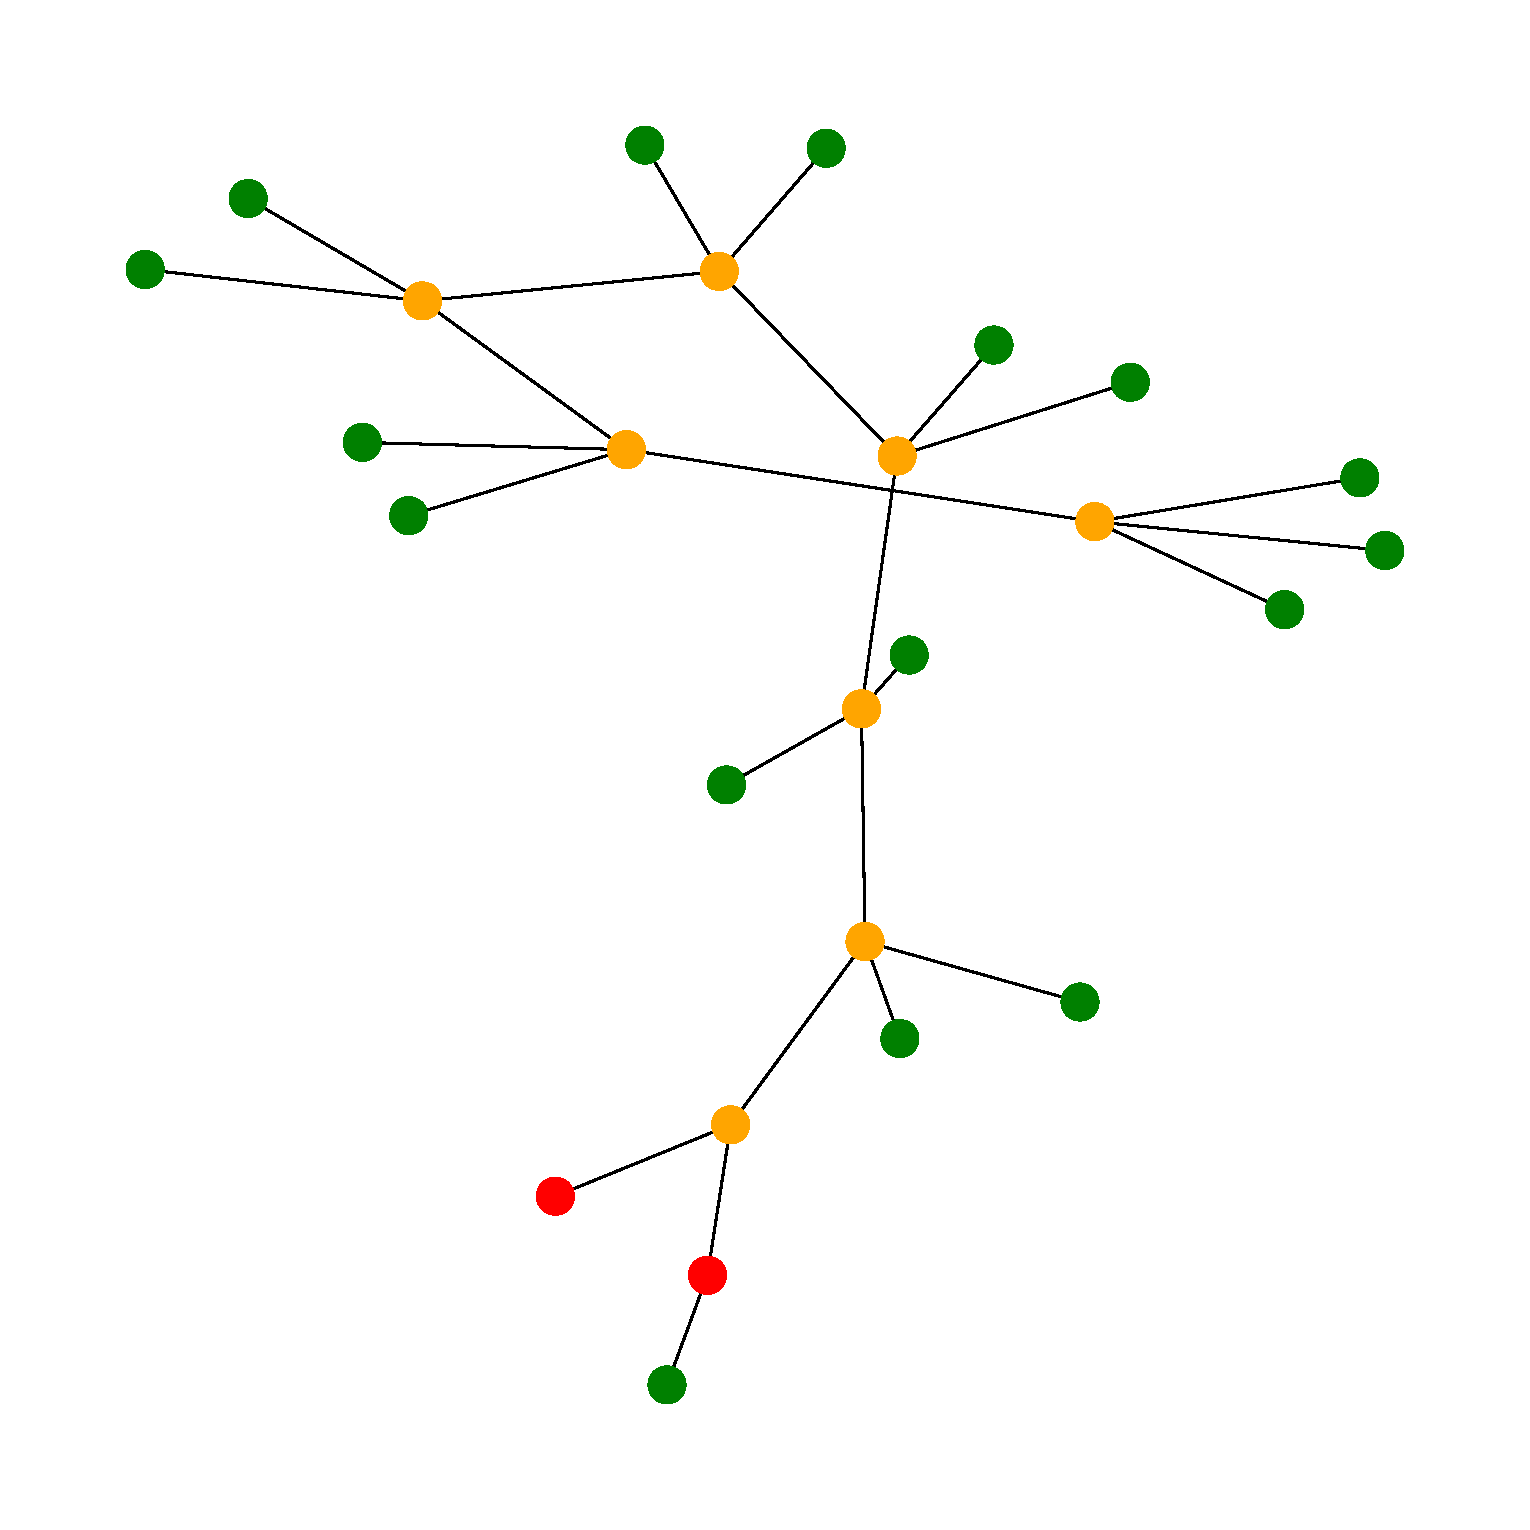
\includegraphics[width=\textwidth]{img/MUTAG-VIS-LARGE-UNLABELED.pdf}
        \caption{MUTAG}
    \end{subfigure}

    \caption[Visualization of original PGExplainer datasets]{Visualization of all six datasets. For node datasets (a-d) the target prediction node where the computational graph is computed from is colored in light blue.}
\end{figure}

\section{Replication Hyperparameter Searches}
\label{sec:sweeps}
The following tables contain the grid search configurations for the explainer on each downstream model. The first row includes the configuration used in the original codebase \cite{luo2020parameterized} and the second row contains the configurations used in \cite{holdijk2021re}. For BA-Community (see Table \ref{tab:BA-Community_sweep}) both configurations are identical, and the second row is thus omitted. The last section of each table contains the set of the values that we tested for each parameter. The optimal settings for our explainer implementation are highlighted in each column. Note that we optimize Tree-Cycles (see Table \ref{tab:Tree-Cycles_sweep}) and BA-2Motif (see Table \ref{tab:BA-2M-sweep}) towards a minimal metric score, as discussed in Section \ref{sec:ind_results}.

\newcolumntype{Y}{>{\centering\arraybackslash}X}
\begin{table}[h]
  \centering
  \scriptsize
  \begin{tabular}{|c|c|c|c|c|c|c|c|c|c|}
  \hline
  \multicolumn{10}{|c|}{\textbf{BA-Shapes}} \\ \hline
  $a$ & $K$ & $b$ & $E$ & $\eta$ & $S$ & $\alpha_e$ & $\alpha_s$ & $\tau_0$ & $\tau_T$ \\ \hline
  $N$ & 1 & 0.0 & 10 & 0.003 & - & 1.0 & 0.05 & 1.0 & 0.05 \\ \hline
  $N$ & 1 & 0.0 & 10 & 0.003 & - & 1.0 & 0.05 & 5.0 & 2.0 \\ \hline
  5 & \textbf{1} & 0.0 & 10 & 0.0003 & 74 & \textbf{0.1} & 0.005 & 5.0 & \textbf{1} \\
   & 5 &  &  & \textbf{0.003} & 75 & 0.5 & \textbf{0.05} &  & 2 \\
   & 10 &  &  & 0.03 & 76 & 1.0 & 0.1 &  & 5 \\ \hline
  \end{tabular}
  \caption[BA-Shapes Grid Search]{First two rows show hyperparameter settings used in \cite{luo2020parameterized} and \cite{holdijk2021re}, respectively. Last section contains our grid search configuration. Bolded values indicate the best performance.}
\end{table}

\begin{table}[h]
  \centering
  \scriptsize
  \begin{tabular}{|c|c|c|c|c|c|c|c|c|c|}
  \hline
  \multicolumn{10}{|c|}{\textbf{BA-Community}} \\ \hline
  $a$ & $K$ & $b$ & $E$ & $\eta$ & $S$ & $\alpha_e$ & $\alpha_s$ & $\tau_0$ & $\tau_T$ \\ \hline
  $N$ & 1 & 0.5 & 20 & 0.003 & - & 1.0 & 0.05 & 1.0 & 1.0 \\ \hline
  64 & 1 & \textbf{0.0} & 20 & \textbf{0.003} & 74 & \textbf{1.0} & 0.05 & 1.0 & 1.0 \\
   & \textbf{5} & 0.5 &  & 0.0003 & 75 & 0.1 & \textbf{0.1} &  & \textbf{5.0} \\
   & 10 &  &  &  & 76 &  &  &  &  \\ \hline
  \end{tabular}
  \caption[BA-Community Grid Search]{First row shows hyperparameter settings used in \cite{luo2020parameterized} and \cite{holdijk2021re}. Last section contains our grid search configuration. Bolded values indicate the best performance.}
  \label{tab:BA-Community_sweep}
\end{table}

\begin{table}[h]
  \centering
  \scriptsize
  \begin{tabular}{|c|c|c|c|c|c|c|c|c|c|}
  \hline
  \multicolumn{10}{|c|}{\textbf{Tree-Cycles}} \\ \hline
  $a$ & $K$ & $b$ & $E$ & $\eta$ & $S$ & $\alpha_e$ & $\alpha_s$ & $\tau_0$ & $\tau_T$ \\ \hline
  $N$ & 1 & 0.0 & 20 & 0.003 & - & 0.01 & 0.0001 & 5.0 & 5.0 \\ \hline
  $N$ & 1 & 0.0 & 20 & 0.003 & - & 10.0 & 0.1 & 1.0 & 5.0 \\ \midrule
  5 & 1 & 0.0 & 20 & \textbf{0.0003} & 74 & 0.01 & \textbf{0.0001} & 1.0 & \textbf{1.0} \\
   & \textbf{5} &  &  & 0.003 & 75 & \textbf{1.0} & 0.05 &  & 5.0 \\
   & 10 &  &  &  & 76 & 10.0 & 0.1 &  &  \\ \hline
  \end{tabular}
  \caption[Tree-Cycles Grid Search]{First two rows show hyperparameter settings used in \cite{luo2020parameterized} and \cite{holdijk2021re}, respectively. Last section contains our grid search configuration. Bolded values indicate the best performance.}
  \label{tab:Tree-Cycles_sweep}
\end{table}

\begin{table}[h]
  \centering
  \scriptsize
  \begin{tabular}{|c|c|c|c|c|c|c|c|c|c|}
  \hline
  \multicolumn{10}{|c|}{\textbf{Tree-Grid}} \\ \hline
  $a$ & $K$ & $b$ & $E$ & $\eta$ & $S$ & $\alpha_e$ & $\alpha_s$ & $\tau_0$ & $\tau_T$ \\ \hline
  $N$ & 1 & 0.0 & 30 & 0.01 & - & 1.0 & 0.01 & 5.0 & 5.0 \\ \hline
  $N$ & 1 & 0.0 & 30 & 0.003 & - & 1.0 & 1.0 & 5.0 & 2.0 \\ \midrule
  24 & 1 & 0.0 & 30 & 0.0003 & 74 & 0.1 & 0.01 & 5.0 & \textbf{2.0} \\
   & \textbf{5} &  & 30 & \textbf{0.003} & 75 & \textbf{1.0} & \textbf{0.5} &  & 5.0 \\
   & 10 &  & 30 & 0.01 & 76 & 10 & 1.0 &  &  \\ 
   &  &  &  & 0.05 &  &  &  &  &  \\ \hline
  \end{tabular}
  \caption[Tree-Grid Grid Search]{First two rows show hyperparameter settings used in \cite{luo2020parameterized} and \cite{holdijk2021re}, respectively. Last section contains our grid search configuration. Bolded values indicate the best performance.}
\end{table}

\begin{table}[h]
  \centering
  \scriptsize
  \begin{tabular}{|c|c|c|c|c|c|c|c|c|c|}
  \hline
  \multicolumn{10}{|c|}{\textbf{BA-2Motif}} \\ \hline
  $a$ & $K$ & $b$ & $E$ & $\eta$ & $S$ & $\alpha_e$ & $\alpha_s$ & $\tau_0$ & $\tau_T$ \\ \hline
  $N$ & 1 & 0.0 & 10 & 0.003 & - & 0.0 & 0.00 & 1.0 & 0.0 \\ \hline
  $N$ & 1 & 0.0 & 20 & 0.005 & - & 0.01 & 0.03 & 5.0 & 1.0 \\ \midrule
  30 & 1 & 0.0 & 10 & 0.0003 & 74 & 0.01 & 0.03 & 5.0 & \textbf{1.0} \\
   & 5 &  & \textbf{20} & 0.003 & 75 & \textbf{0.1} &  &  & 5.0 \\
   & \textbf{10} &  &  & 0.005 & 76 &  &  &  &  \\
   &  &  &  & \textbf{0.01} &  &  &  &  &  \\ \hline
  \end{tabular}
  \caption[BA-2Motif Grid Search]{First two rows show hyperparameter settings used in \cite{luo2020parameterized} and \cite{holdijk2021re}, respectively. Last section contains our grid search configuration. Bolded values indicate the best performance.}
  \label{tab:BA-2M-sweep}
\end{table}

\begin{table}[h]
  \centering
  \scriptsize
  \begin{tabular}{|c|c|c|c|c|c|c|c|c|c|}
  \hline
  \multicolumn{10}{|c|}{\textbf{MUTAG}} \\ \hline
  $a$ & $K$ & $b$ & $E$ & $\eta$ & $S$ & $\alpha_e$ & $\alpha_s$ & $\tau_0$ & $\tau_T$ \\ \hline
  $N$ & 1 & 0.0 & 10 & 0.01 & - & 1.0 & 0.01 & 5.0 & 5.0 \\ \hline
  $N$ & 1 & 0.0 & 30 & 0.0003 & - & 1.0 & 0.005 & 5.0 & 5.0 \\ \midrule
  30 & 1 & 0.0 & 10 & 0.0003 & 74 & 0.1 & 0.01 & 5.0 & \textbf{1.0} \\
   & 5 &  & \textbf{20} & 0.003 & 75 & \textbf{1.0} & \textbf{0.005} &  & 5.0 \\
   & \textbf{10} &  & 30 & \textbf{0.01} & 76 &  &  &  &  \\ \hline
  \end{tabular}
  \caption[MUTAG Grid Search]{First two rows show hyperparameter settings used in \cite{luo2020parameterized} and \cite{holdijk2021re}, respectively. Last section contains our grid search configuration. Bolded values indicate the best performance.}
\end{table}

\clearpage
\section{Multiple Explanation Visualizations}
\label{sec:grid_vis}
The following figures contain 16 randomly sampled explanations for the best explainer model of every dataset. For graph tasks all nodes of the input graph are included, while for node tasks only the nodes of the local computation graph from the prediction motif node are shown.

% REMOVE draw=black TO REMOVE EDGES
\begin{figure}[htbp]
    \centering
    \begin{tikzpicture}
      % 4x4 grid: row = 0 to 3, col = 0 to 3
      \foreach \row in {0,...,3} {
        \foreach \col in {0,...,3} {
          \pgfmathtruncatemacro{\num}{\col + 4 * \row}
          \node[draw=black, thin, inner sep=0pt] at (\col*4, -\row*4)
            {\includegraphics[width=3.5cm]{img/BA-Shapes/graph_\num_explanation.pdf}};
        }
      }
    \end{tikzpicture}
    \caption{Grid of BA-Shapes explanations (top-6 edges)}
    \label{fig:grid-BA-Shapes-explanations}
\end{figure}

\begin{figure}[htbp]
    \centering
    \begin{tikzpicture}
      % 4x4 grid: row = 0 to 3, col = 0 to 3
      \foreach \row in {0,...,3} {
        \foreach \col in {0,...,3} {
          \pgfmathtruncatemacro{\num}{\col + 4 * \row}
          \node[draw=black, thin, inner sep=0pt] at (\col*4, -\row*4)
            {\includegraphics[width=3.5cm]{img/BA-Community/graph_\num_explanation.pdf}};
        }
      }
    \end{tikzpicture}
    \caption{Grid of BA-Community explanations (top-6 edges)}
    \label{fig:grid-BA-Community-explanations}
\end{figure}

\begin{figure}[htbp]
    \centering
    \begin{tikzpicture}
      % 4x4 grid: row = 0 to 3, col = 0 to 3
      \foreach \row in {0,...,3} {
        \foreach \col in {0,...,3} {
          \pgfmathtruncatemacro{\num}{\col + 4 * \row}
          \node[draw=black, thin, inner sep=0pt] at (\col*4, -\row*4)
            {\includegraphics[width=3.5cm]{img/Tree-Cycles/graph_\num_explanation.pdf}};
        }
      }
    \end{tikzpicture}
    \caption{Grid of Tree-Cycles explanations (top-6 edges)}
    \label{fig:grid-Tree-Cycles-explanations}
\end{figure}

\begin{figure}[htbp]
    \centering
    \begin{tikzpicture}
      % 4x4 grid: row = 0 to 3, col = 0 to 3
      \foreach \row in {0,...,3} {
        \foreach \col in {0,...,3} {
          \pgfmathtruncatemacro{\num}{\col + 4 * \row}
          \node[draw=black, thin, inner sep=0pt] at (\col*4, -\row*4)
            {\includegraphics[width=3.5cm]{img/Tree-Grid/graph_\num_explanation.pdf}};
        }
      }
    \end{tikzpicture}
    \caption{Grid of Tree-Grid explanations (top-12 edges)}
    \label{fig:grid-Tree-Grid-explanations}
\end{figure}

\begin{figure}[htbp]
    \centering
    \begin{tikzpicture}
      % 4x4 grid: row = 0 to 3, col = 0 to 3
      \foreach \row in {0,...,3} {
        \foreach \col in {0,...,3} {
          \pgfmathtruncatemacro{\num}{\col + 4 * \row}
          \node[draw=black, thin, inner sep=0pt] at (\col*4, -\row*4)
            {\includegraphics[width=3.5cm]{img/BA-2Motif/graph_\num_explanation.pdf}};
        }
      }
    \end{tikzpicture}
    \caption{Grid of BA-2Motif explanations (top-5 edges)}
    \label{fig:grid-BA-2Motif-explanations}
\end{figure}

\begin{figure}[htbp]
    \centering
    \begin{tikzpicture}
      % 4x4 grid: row = 0 to 3, col = 0 to 3
      \foreach \row in {0,...,3} {
        \foreach \col in {0,...,3} {
          \pgfmathtruncatemacro{\num}{\col + 4 * \row}
          \node[draw=black, thin, inner sep=0pt] at (\col*4, -\row*4)
            {\includegraphics[width=3.5cm]{img/MUTAG/graph_\num_explanation.pdf}};
        }
      }
    \end{tikzpicture}
    \caption{Grid of MUTAG explanations (top-10 edges)}
    \label{fig:grid-MUTAG-explanations}
\end{figure}

\clearpage
\section{NeuroSAT explainer Hyperparameter Searches}

The following tables contain the grid search configurations for the NeuroSAT explainer models with either the soft constraint or the hard constraint applied. The columns contain the values tested for the corresponding hyperparameter. The optimal settings for each explainer implementation are highlighted.

For the hard constraint the mean local ROC-AUC was no higher than $0.502$ and no lower than $0.44$ over all runs. We select the hyperparameters that maximize the metric and minimize the validation loss while avoiding edge weights of 0. TODO:

We conclude that regardless of exact hyperparameters, the NeuroSAT model does not succinctly learn UNSAT cores.


\begin{table}[h]
  \centering
  \scriptsize
  \begin{tabular}{|c|c|c|c|c|c|c|c|c|c|c|}
  \hline
  \multicolumn{11}{|c|}{\textbf{Soft Constraint Explainer}} \\ \hline
  $\alpha_e$ & $E$ & $\eta$ & $K$ & $\alpha_{concat}$ & $S$ & $\alpha_s$ & $\tau_T$ & $\tau_0$ & $\alpha_{C}$ & $\alpha_{AdamW}$ \\ \hline
  0.1 & \textbf{20} & \textbf{0.0003} & 1 & False & 75 & \textbf{0.001} & \textbf{1.0} & 5.0 & 0.1 & False\\ 
  \textbf{1.0} & 30 & 0.003 & \textbf{5} & \textbf{True} & 76 & 0.01 & 5.0 &  & 1.0 & \textbf{True}\\ 
   & 50 & 0.01 &  &  &  & 0.1 &  &  & \textbf{10.0} & \\ \hline
  \end{tabular}
  \caption[NeuroSAT soft constraint Sweep]{Grid search results over hyperparameter space for the NeuroSAT explainer that uses a soft constraint. Bolded values indicate the best performance.}
\end{table}

\begin{figure}
  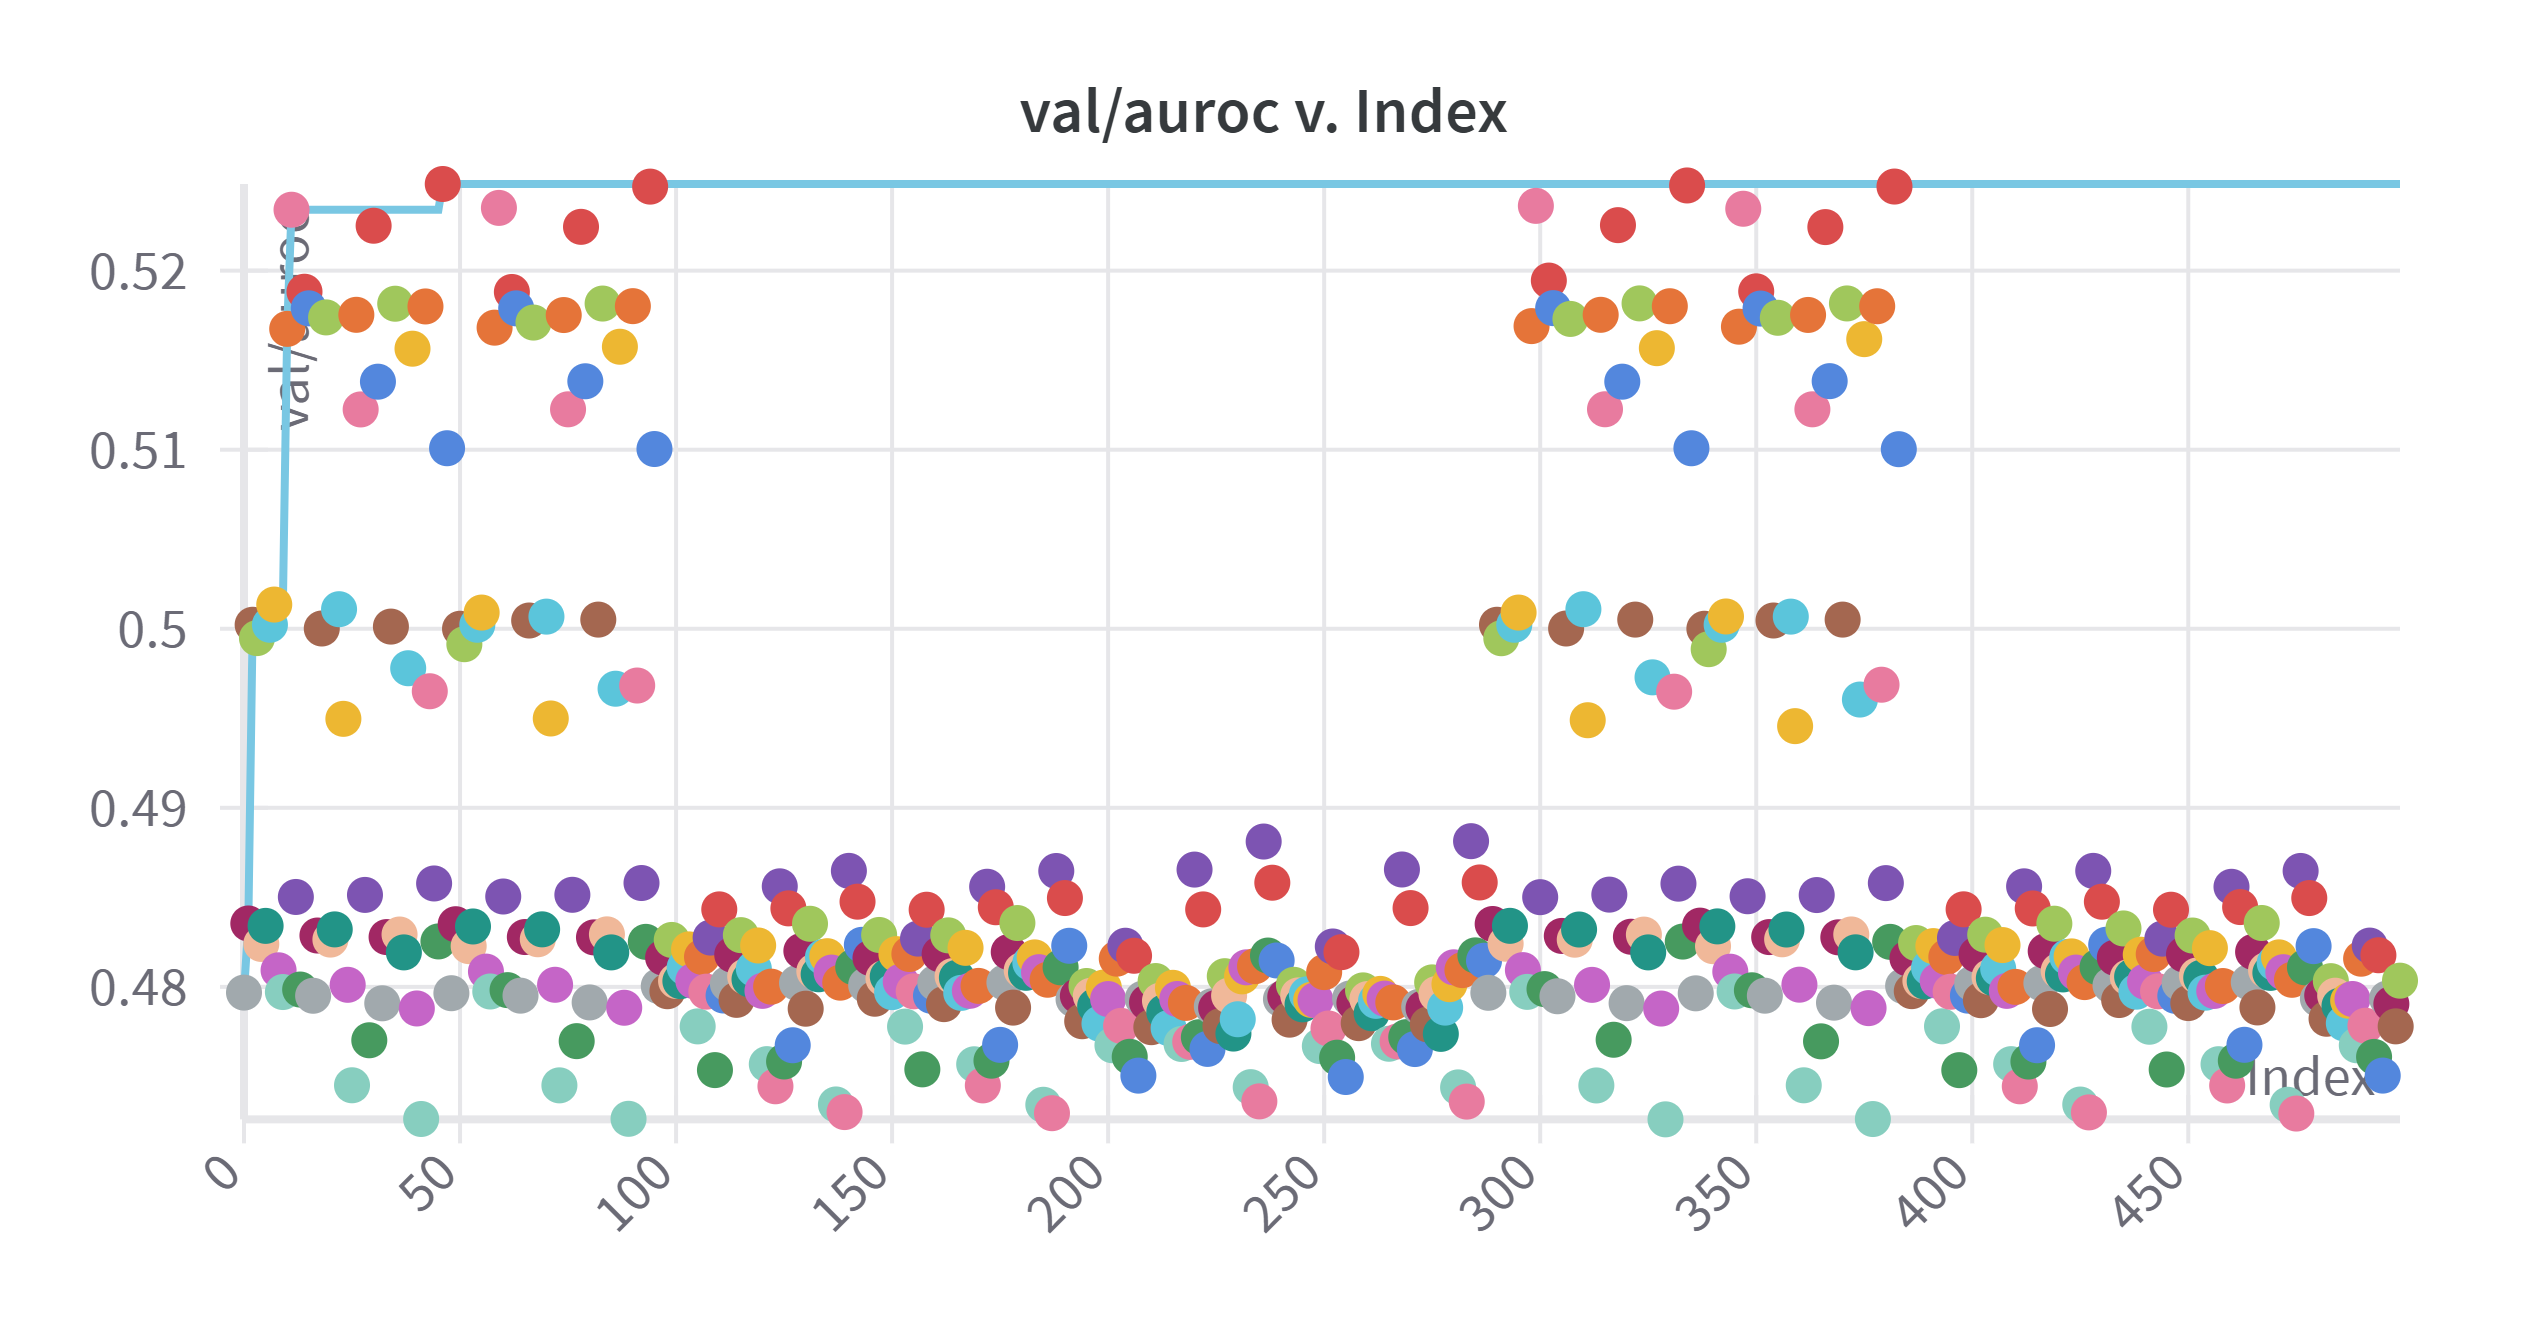
\includegraphics[width=\linewidth]{img/NeuroSAT-soft_sweep.png}
  \caption{Grid search results of all runs using WandB \cite{}.}
\end{figure}



\begin{table}[h]
    \centering
    \scriptsize
    \begin{tabular}{|c|c|c|c|c|c|c|c|c|c|}
    \hline
    \multicolumn{10}{|c|}{\textbf{Hard Constraint Explainer}} \\ \hline
    $\alpha_e$ & $E$ & $\eta$ & $K$ & $\alpha_{concat}$ & $S$ & $\alpha_s$ & $\tau_T$ & $\tau_0$ & $\alpha_{arch}$ \\ \hline
    0.1 & 20 & \textbf{0.0003} & 1  & \textbf{False} & 75 & \textbf{0.01} & \textbf{1.0} & 5.0 & False \\
    \textbf{1.0} & 30 & 0.003  & \textbf{5}  & True  & 76 & 0.1 & 5.0 &  & \textbf{True}  \\
        &  \textbf{50} & 0.01   &  &       &     &   1.0   &      &      &       \\ \hline
    \end{tabular}
    \caption[NeuroSAT hard constraint Sweep]{TODO: ALSO INCLUDE LOWER LR?!?! Highlighted values are the best performing ones, leading to a smaller mean validation AUROC and avoiding same weighted edges. Bolded values indicate the best performance.
    }
\end{table}

\newpage
\section{REMOVE}
\begin{table}[ht]
  \centering
  \scriptsize
  \begin{tabularx}{\textwidth}{l*{4}{X}}   % Now only 4 datasets
  \toprule
  \textbf{} & \multicolumn{4}{c}{\textbf{Explanation AUC}} \\
  \cmidrule{2-5}
  \textbf{Method} & BA-Shapes & BA-Community & Tree-Cycles & Tree-Grid \\
  \midrule
  Our work (inductive) & 0.993$\pm$0.002 & 0.829$\pm$0.008 & 0.109$\pm$0.108 & 0.689$\pm$0.027 \\
  \addlinespace
  \midrule
  \midrule
  \textit{Inference Time (ms)} & 39.0$\pm$1.9 & 25.6$\pm$1.5 & 3.1$\pm$0.3 & 3.4$\pm$0.1 \\
  \bottomrule
  \end{tabularx}
  \caption[REMOVE! PGExplainer with $a=0.08$!]{PGExplainer performance WITH $a=0.08$! (4.8, 64, 4.8, 23) (USED IN SWEEP!)}
  \label{tab:rem1}
\end{table}


\begin{figure}[htbp]
    \centering
    \begin{minipage}{0.48\textwidth}
        \centering
        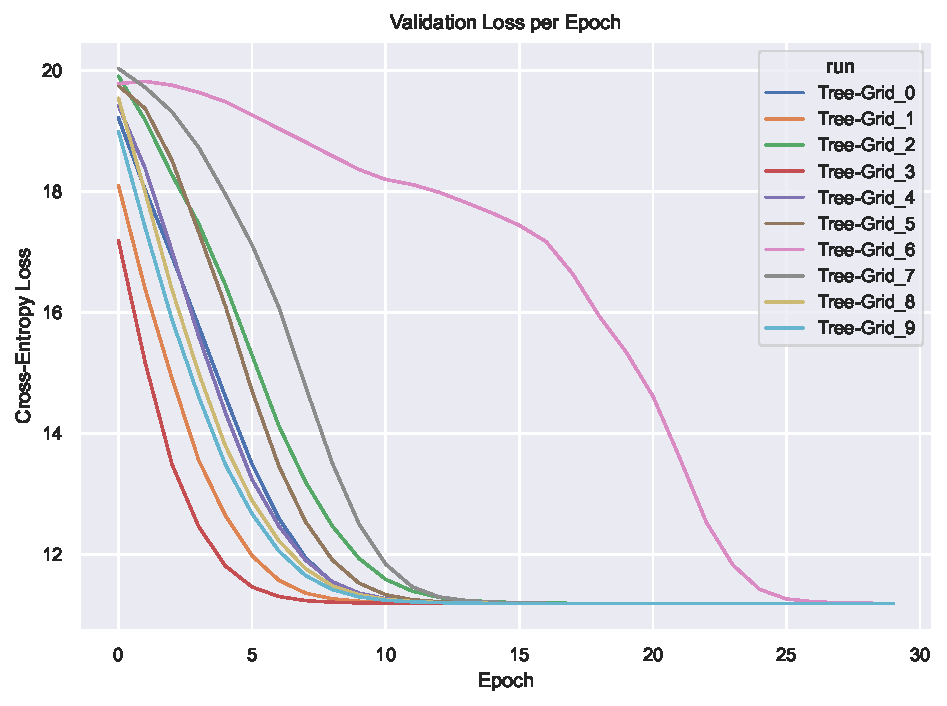
\includegraphics[width=\textwidth]{img/plots/Grid_val_loss_plot.pdf}  % Plot 1
        \caption{Mean validation Loss per Epoch (Tree-Grid).}
        \label{fig:Tree-Grid-val_loss}
    \end{minipage}
    \hfill
    \begin{minipage}{0.48\textwidth}
        \centering
        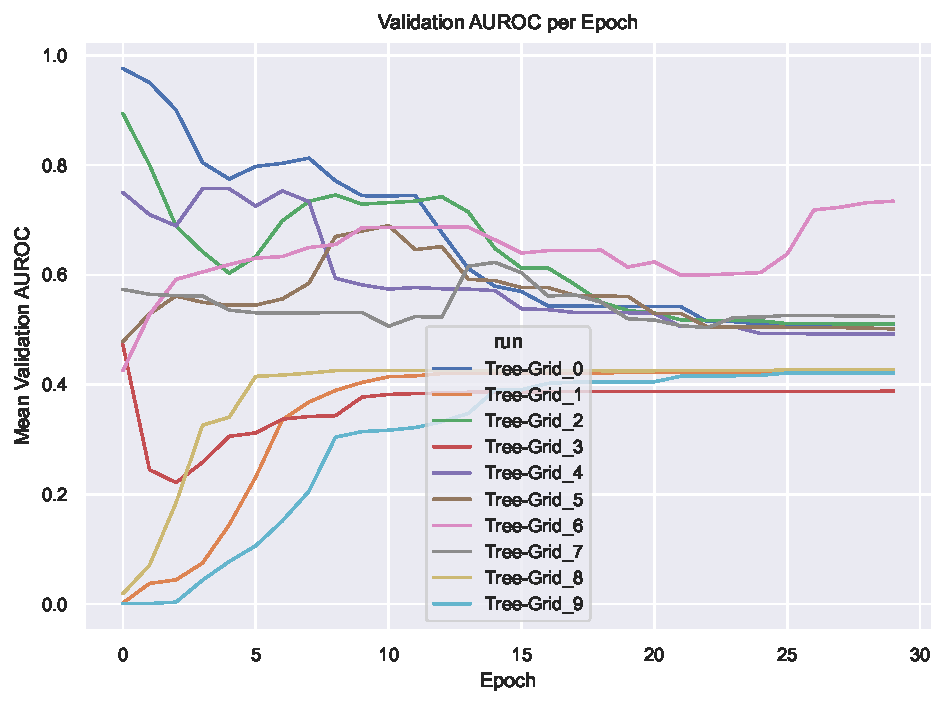
\includegraphics[width=\textwidth]{img/plots/Grid_val_auroc_plot.pdf}  % Plot 2
        \caption{Mean validation AUROC per Epoch (Tree-Grid).}
        \label{fig:Tree-Grid-val_auroc}
    \end{minipage}
\end{figure}


    % Second part without vertical lines
    \begin{tabular}{l|cccc}
    \midrule
    \textbf{} & \multicolumn{4}{c}{\textbf{One-Motif-Node-Train}} \\
    \addlinespace
    \toprule
    \#used motif instances $N$ & 60 & 60 & 160  & 32 \\
    \bottomrule
    \end{tabular}

  

\begin{table}[ht]
    \centering
    \scriptsize
    \begin{tabularx}{0.6\textwidth}{l*{4}{X}}   % Adjust width as needed
    \toprule
    \textbf{} & \multicolumn{4}{c}{\textbf{Explanation AUROC}} \\
    \cmidrule{2-5}
    \textbf{Method} & BA-Shapes & BA-Community & Tree-Cycles & Tree-Grid \\
    \midrule
    Experiment & 0.85$\pm$0.005 & 0.731$\pm$0.016 & 0.224$\pm$0.160 & 0.65$\pm$0.026 \\
    \bottomrule
    \end{tabularx}
    \caption[REM]{TODO: THIS DOES NOT MAKE SENSE! TRAIN AND EVAL NODES SHALL BE FROM THE SAME DISTRIBUTION!!! Explanation AUROC for One-Motif-Node-Train.}
    \label{tab:allmotifnodes_selected_rem}
\end{table}